\documentclass[11pt]{article}
\usepackage[utf8x]{inputenc}
\usepackage[english]{babel}
\usepackage{graphicx}
\usepackage{wrapfig}
\usepackage[margin=1.5cm, tmargin=2cm]{geometry}
\usepackage{color}
\usepackage{hyperref}
\usepackage{paralist}
\usepackage{wrapfig}
\usepackage{multicol}

\begin{document}
\noindent First name: \hfill INFO2, ENSIBS Vannes, 2014-12-17\\
Last name:
\begin{center}
	{\LARGE{Network evaluation}} \\
	All documents are allowed, but no communication at all!\\
	\textbf{Short} and right answers are the best (French or English). No need to debate, nor philosophize.\\
	Good luck!
\end{center}
\vspace{-22pt}
\section{OSI model (2 pts)}\vspace{-11pt}
Give the name and a short overview of the four first layers' objectives (without details):
\vspace{7cm}
\section{Domain Name System (2 pts)}\vspace{-11pt}
Theses packets were captured on my laptop just after a \verb_ping_.
\begin{figure}[h!]
	\begin{tabular}{c|cc|c|p{8cm}}
		\textbf{Number} & \textbf{Source} & \textbf{Destination} & \textbf{Protocol} & \textbf{Comment} \\ \hline
		1 & 192.168.0.1 & 208.67.222.222 & DNS & Standard query 0xb559  A imdb.com \\
		2 &	208.67.222.222 & 192.168.0.1 & DNS & Standard query response 0xb559 A 207.171.166.22 A 72.21.210.29 A 72.21.206.80 
	\end{tabular}
	\caption{DNS query}
\end{figure}
\vspace{-22pt}
\begin{itemize}
	\item What is my IP address?
	\item What is my DNS server IP address?
	\item What could be the destination(s) of the $ping$?
	\item What is the domain name I tried to $ping$?
\end{itemize}

\begin{wrapfigure}{r}{0.5\textwidth}
   \vspace{-40pt}
   \begin{center}
    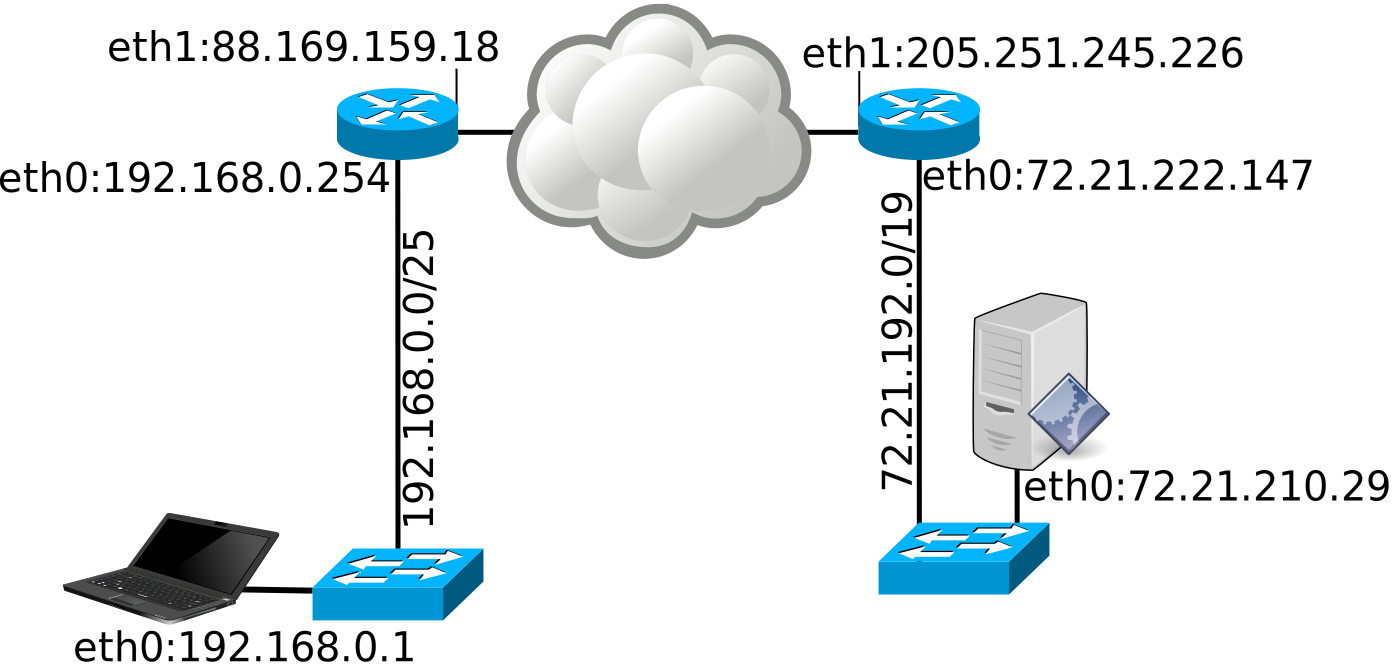
\includegraphics[width=0.5\textwidth]{./ntwk.pdf}
   \end{center}
   \vspace{-10pt}
  \caption{Buggy network}
     \vspace{-90pt}
  \label{bgg-ntwk}
\end{wrapfigure}


\section{Debug it (5 pts)}\vspace{-11pt}
Using the output of the following commands, correct the network displayed in fig.\ref{bgg-ntwk}. \\
\verb+ $ping 72.21.206.80+ \\
\verb+  Host Unreachable+ \\
\verb+ $route -n + \\
\begin{tabular}{lll}
	\verb+Destination+ & \verb+Gateway+ & \verb+Genmask+ \\
	\verb+0.0.0.0+ 			 & \verb+192.168.0.3+		& \verb+0.0.0.0+ \\
	\verb+192.168.0.0+			 & \verb+0.0.0.0+			& \verb+255.255.255.0+ \\
\end{tabular}


\pagebreak
\setlength{\columnseprule}{1pt}
\section{Design it (11 pts)}\vspace{-11pt}
\begin{multicols}{2}
	In this question you need to design several subnetworks. Starting from 176.22.0.0, give for each single subnetwork (no schema expected):
	\begin{itemize}
		\item the subnet mask and maximum number of hosts,
		\item the network IP address,
		\item the first node IP address,
		\item the last node IP address,
		\item the broadcast IP address,
		\item the CIDR of the "super-network".
	\end{itemize}
\vspace{11pt}	Sub-networks to be desgined are:
	\begin{enumerate}[a.]
		\item 10000 machines for the students,
		\item 300 machines for the network services (DNS server, web, NAS...),
		\item 200 machines for the IT administration,
		\item 50 machines for the network lab,
		\item 1000 machines for the teachers and workers.
	\end{enumerate}

\end{multicols}


\end{document}
